%& --translate-file=cp1250pl
%bez powyzszej linijki nie dzialaja polskie znaki (musi ona byc w pierwszej linii dokumentu
%%&platex --translate-file=il2-pl % przeyestowac z tym
\documentclass[a4paper,12pt]{article}
\usepackage[english]{babel}
\usepackage[T1]{fontenc}
\usepackage[dvips]{graphicx}
%\usepackage{intendfirst}
\usepackage{times}
\usepackage{epsfig}
\usepackage{color}
\usepackage[urlcolor=blue, colorlinks=true, bookmarks=true, bookmarksnumbered=true]{hyperref}

\usepackage{fancyhdr} 
\pagestyle{fancy} 

\rfoot{SALOMON}


%ustawienie wielkosci akapitu
%\setlength{\parindent}{0mm}
%%odst�p mi�dzy akapitami
%\setlength{\parskip}{2mm}

%ustawienia rozmiaru tekstu
    \textwidth 16cm
    \textheight 24cm 
    \topmargin -15mm
    \evensidemargin-3mm
    \oddsidemargin -3mm
    


\title{Introduction to Salomon}

\author{Nikodem Jura \emph{(nico@icslab.agh.edu.pl)}
        \\
        Krzysztof Rajda \emph{(krzycho@student.uci.agh.edu.pl)}
        \\
        Jakub Ga�kowski \emph{(avi@student.uci.agh.edu.pl)}               
        \\
        Jakub Paw�owski \emph{(qoooba@student.uci.agh.edu.pl)}}             
        

\begin{document}

\maketitle
%wylaczenie numerowania na I stronie
\thispagestyle{empty}

\begin{center}
\href{http://salomon.iisg.agh.edu.pl}{http://salomon.iisg.agh.edu.pl}
\end{center}

\pagebreak
\section{Intro}

Salomon is a system for extracting knowledge out of data using \emph{Knowledge Mining} methodology.

\subsection{Goal}

The goal of this project is to create a friendly environment for creating, controlling and effective performing of tasks and storing collected knowledge.

\subsection{Assumptions}

Basic design objectives:
\begin{itemize}
	\item \textbf{all functionality in plug-ins.}
	
	The core of the system should be as light as possible. Its goal is to create an environment for realizing the functionality provided with the plug-ins.
	
	\item \textbf{open architecture.}
	
	Inserting a middle tier between database and plug-ins. Its goal is to hide the details of how the data is organized. Architecture openness gives the possibility to extend this tier.
	
	\item \textbf{platform independence.}
	
	System should be platform independent and easily portable. Thus each part of the system can be run on different operating systems.
	\item \textbf{possibility of using the results of some task by consequent tasks.}
	\item \textbf{ easy adaptation of the functionality contained in \emph{Vinlen}.}
	
	Project has been originally designed to be a platform for running the logics implemented in \emph{Vinlen} program,
	created under supervision of Prof. Ryszard Michalski
	
\end{itemize}

\begin{figure}[ht]
	\centering
		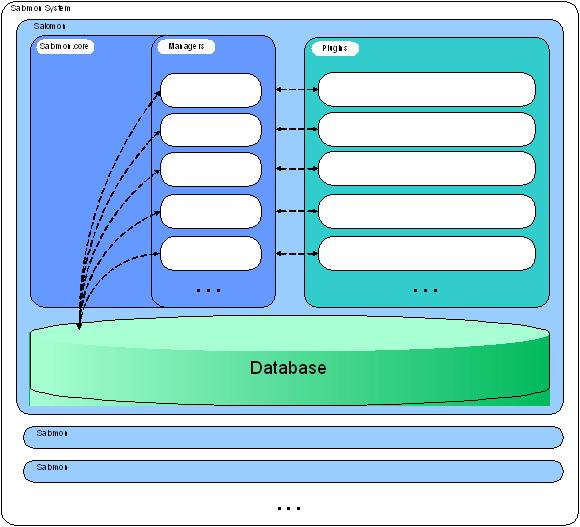
\includegraphics[width=0.70\textwidth]{img/uml/arch.jpg}
	\caption{System architecture}
\end{figure}

\newpage
\section{Knowledge processing}

\subsection{Graph}

Discovering knowledge is an iterative, divided into stages, process. Stages can form cycles. 
During each stage the knowledge is processed. Knowledge discovering process can be directed according to the user's preferences. Each stage forms a closed whole. Some stages are separate, so they can be performed concurrently. Salomon's architecture enables support for distributed (and this implies concurrent) processing of those stages and synchronizing their results.

The representation of the stage in Salomon is a \emph{task}. Each task may have a few predecessors and consequents. Simply speaking, tasks can be organized in a form of a graph.

The task is defined as a triple:
\begin{itemize}
	\item algorithm (provided in a form of a plug-in)
	\item data which controls the algorithm
	\item entry data, out of which the algorithm extracts the knowledge
\end{itemize}

\begin{figure}[ht]
	\centering
		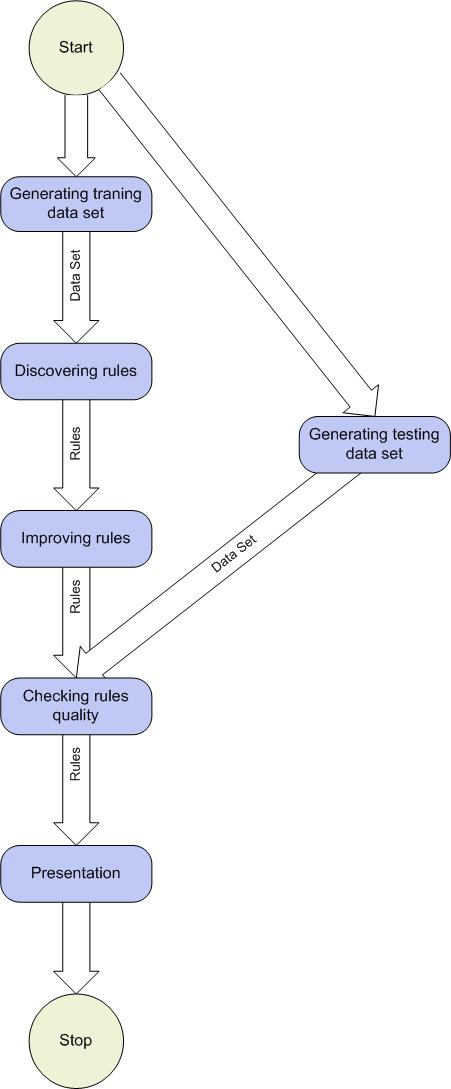
\includegraphics[height=0.4\textheight]{img/concept/WorkflowGraph.jpg}
	\caption{General workflow}
	\label{fig:WorkflowGraph}
\end{figure}

\subsection{Task}

The task does not have to be limited to the data, provided by the previous task. Each task has access to the whole currently gathered knowledge and to all data. 

In the output or input of each task there can be data (in case of algorithms, which filters and organize data), knowledge or both of these at the same time.
\begin{itemize}
	\item data \begin{math}\Rightarrow \end{math} data - this case occurs most often when we want to create training or test sets
	\item data \begin{math}\Rightarrow \end{math} knowledge - typical example of knowledge mining: we are given with data, and return knowledge
	\item data + knowledge \begin{math}\Rightarrow \end{math} data - this case occurs when we want to use collected knowledge on the given data
	\item knowledge \begin{math}\Rightarrow \end{math} knowledge
\end{itemize}

\subsection{Differences to Vinlen}

Salomon is meant to eliminate the limits of original \emph{Vinlen} by introducing:
\begin{itemize}
	\item queuing of tasks
	\item distribution
	\item concurrency
	\item extendability (plug-ins mechanism)
	\item portability (Java\texttrademark, Firebird)
\end{itemize}

\newpage
\section{Technical details}

\textit{Salomon} consists of environment (core) and plug-ins:
\begin{itemize}
	\item \textbf{Core} manages and distributes tasks as well  as gives environment in which plug-ins operate.
	\item \textbf{Plug-ins} are responsible for operating on data, knowledge creation, displaying results etc. They implement logic of the specified task. They can be dynamically loaded and unloaded.
\end{itemize}

Thanks to the core plug-ins are separated from details of implementation and operate on very high level of abstraction using API given by the core.

Interaction with user can be implemented in various ways: as a standalone application, distributed system, agent system, a library which can be used by other programs, etc. This layer(presentation layer) is very flexible and can be easily extended. User can also switch between different presentation views.

Thanks to \textit{Salomon} we can implement iterative learning model(one of the basic concepts of knowledge mining) which assumes that knowledge created in one iteration can be used for knowledge creation in the other one.

\textit{Salomon} enables the communication between tasks. For example: we create at the beginning a learning set, first plug-in extracts some rules from this set which are later enhanced by other plug-ins. At the end the last plug-in presents the results to the user.


Tasks can be connected(by pipes), they can create loops and generally they can be organized in a graph. Because database layer is separated from plug-ins, databases do not have to be exactly the same, they only need to have common attributes defined in our API. If we have for example some databases in hospitals which store data about patients, diseases etc. we do not need to synchronize them and change their format, plug-ins can extract knowledge from what is available for them and thanks to distribution of \textit{Salomon} share with other plug-ins everything they have learned.

\textit{Salomon} is portable between different operating systems(Windows, Linux, MacOS, Solaris, FreeBSD, etc.). We have also put a lot of effort in ensuring integrity of data, so all operations are atomic and treated as a transaction - if something fails, all changes made by this operation until the failure are rolled back.

\newpage
\section{Acknowledgments}

	Inspiration for creating project ,,Salomon,, was the presentation shown by Prof. Ryszard Michalski, which concerned the system \emph{Vinlen}. 

\end{document}
